\documentclass[12pt]{article}
\usepackage{amsmath}
\usepackage{array}
% \usepackage{gensymb}
\usepackage{geometry}
\usepackage{graphicx}
\usepackage{pgfplots}
\usepackage{siunitx}
\usepackage{wrapfig}

\title{Homework \#10}
\author{Donald Aingworth IV}
\date{October 30, 2024}

\pgfplotsset{width=8cm,compat=1.9}
\usepgfplotslibrary{external}
% \tikzexternalize

\begin{document}

\DeclareSIUnit{\mile}{mi}
\DeclareSIUnit{\gal}{gal}
\DeclareSIUnit{\foot}{ft}
\DeclareSIUnit{\h}{h}

\maketitle

\pagebreak
\section*{Problem 1}
A 1.95-kg particle is projected with an initial speed of 4.00 m/s along a surface for which $\mu_k = 0.600$. Find the distance it travels given that: (a) the surface is horizontal; (b) the particle moves up a 30\unit{\degree} incline; (c) the particle moves down a 30\unit{\degree} incline.

\subsection*{Solution}
Work is defined by $ W = \vec{F}\cdot\vec{d} $. In this instance, we can use the frictional force to expand this into the kinetic frictional work using g = 9.81\unit{\meter/\second^2}. The friction force will also be antiparallel to the motion in this instance until the block stops.
\begin{align*}
    W_k &=  \vec{f_k}\cdot\vec{d}
        =   f_k*d*\cos(180\unit{\degree})
        =   -f_k*d\\
        &=  -\mu_k*F_N*d
        =   -\mu_k*m*g*d
\end{align*}
We next can calculate the work done by gravity.
\begin{align*}
    W_g &=  \vec{F_g}\cdot\vec{d}
        =   F_g*d*\sin(\theta)
        =   m*g*d*\sin(\theta)
\end{align*}
We use the formula for the kinetic energy.
\begin{align*}
    K   &=  \frac{1}{2}mv^2\\
    \Delta K    &=  K_f - K_i
                =   \frac{1}{2}mv_f^2 - \frac{1}{2}mv_i^2
\end{align*}
We combine these three to get a formula for the distance here. We should place special attention on the formula $K_f = K_i + W_\Sigma$. 
\begin{align*}
    K_f &=  K_i + W_\Sigma
        =   K_i + W_g - W_k\\
    \frac{1}{2}mv_f^2 &= \frac{1}{2}mv_i^2 + m*g*d*\sin(\theta) - \mu_k*m*g*d\\
    \frac{1}{2}(v_f^2 - v_i^2)  &=  d*g*(\sin(\theta)-\mu_k)\\
    d   &=  \frac{v_f^2 - v_i^2}{2*g*(\sin(\theta)-\mu_k)}
\end{align*}
We will call this last formula  "Formula 1", not named after the racecar competition.
\pagebreak
\subsubsection*{Section (a)}
We apply Formula 1.
\begin{align*}
    d   &=  \frac{v_f^2 - v_i^2}{2*g*(\sin(\theta)-\mu_k)}
        =   \frac{(0\unit{\meter/\second})^2 - (4\unit{\meter/\second})^2}{2*(9.81\unit{\meter/\second^2})*(\sin(0\unit{\degree})-0.600)}\\
        &=  \frac{ - 16\unit{\meter^2/\second^2}}{19.62\unit{\meter/\second^2}*(-0.600)}
        =   \frac{16\unit{\meter^2/\second^2}}{11.772\unit{\meter/\second^2}}
        =   \boxed{1.359\unit{\meter}}\\
\end{align*}

\subsubsection*{Section (b)}
We apply Formula 1.
\begin{align*}
    d   &=  \frac{v_f^2 - v_i^2}{2*g*(\sin(\theta)-\mu_k)}
        =   \frac{(0\unit{\meter/\second})^2 - (4\unit{\meter/\second})^2}{2*(9.81\unit{\meter/\second^2})*(\sin(30\unit{\degree})-0.600)}\\
        &=  \frac{ - 16\unit{\meter^2/\second^2}}{19.62\unit{\meter/\second^2}*(0.500-0.600)}
        =   \frac{16\unit{\meter^2/\second^2}}{1.962\unit{\meter/\second^2}}
        =   \boxed{8.155\unit{\meter}}\\
\end{align*}

\subsubsection*{Section (c)}
We apply Formula 1.
\begin{align*}
    d   &=  \frac{v_f^2 - v_i^2}{2*g*(\sin(\theta)-\mu_k)}
        =   \frac{(0\unit{\meter/\second})^2 - (4\unit{\meter/\second})^2}{2*(9.81\unit{\meter/\second^2})*(\sin(-30\unit{\degree})-0.600)}\\
        &=  \frac{ - 16\unit{\meter^2/\second^2}}{19.62\unit{\meter/\second^2}*(-0.500-0.600)}
        =   \frac{16\unit{\meter^2/\second^2}}{21.582\unit{\meter/\second^2}}
        =   \boxed{0.741\unit{\meter}}\\
\end{align*}

\pagebreak
\section*{Problem 2}
% \begin{wrapfigure}{r}{0.35\textwidth}
%     \vspace{-30pt}
%     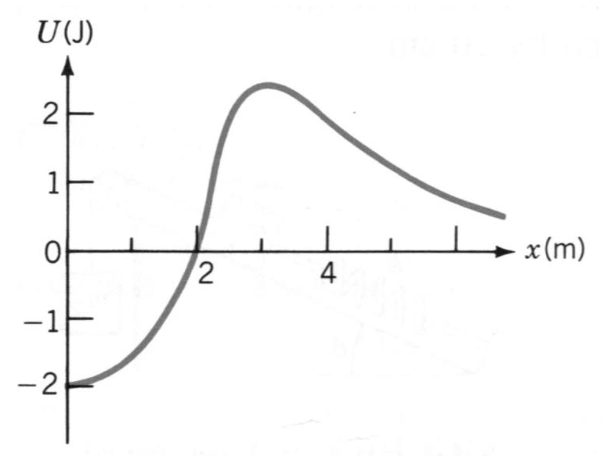
\includegraphics[width=0.35\textwidth]{graph_2.png} 
%     % \label{fig:wrapfig}
% \end{wrapfigure}

% \subsection*{Solution}

\pagebreak
\section*{Problem 3}
\begin{wrapfigure}{r}{0.35\textwidth}
    \vspace{-30pt}
    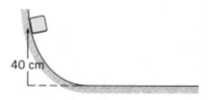
\includegraphics[width=0.35\textwidth]{graph_3.png} 
    % \label{fig:wrapfig}
\end{wrapfigure}
A 1.75-kg block starts from rest at an initial height of 40.0 cm and slides down a frictionless circular ramp, as shown in the figure below. It slides for 79.0 cm on the horizontal surface before coming to a stop. What is the coefficient of kinetic friction? Assume that only the horizontal stretch has friction, and the curved portion is frictionless.

\subsection*{Solution}
First, we find the velocity when the block switches from the frictionless to the frictional ground by using the conservation of energy since all energy on the frictionless part is conservative.
\[ K_f - U_f = K_i - U_i \]
\[ \frac{1}{2}mv_f^2 - m*g*y_f = \frac{1}{2}mv_i^2 - m*g*y_i \]
The final y-position is zero, as is the initial velocity.
\[ \frac{1}{2}mv_f^2 = -m*g*y_i \]
\[ v_f^2 = -2*g*y_i \]
We keep in mind that in this instance, $ g = -9.81\unit{\meter/\second^2} $, so we need not here worry about the velocity being imaginary.\\
From here, we can use a kinetic energy and work formula to find the final kinetic energy. We here use that $F_N = -F_g = -mg$.
\begin{align*}
    K_f &=  K_i + W_k\\
    \frac{1}{2}mv_f^2   &=  \frac{1}{2}mv_i^2 - F_N * \mu_k * d
        =   \frac{1}{2}mv_i^2 + m * g * \mu_k * d\\
    g * \mu_k * d   &= \frac{1}{2}(v_f^2 - v_i^2)\\
    \mu_k   &=  \frac{v_f^2 - v_i^2}{2*g*d}
            =   \frac{(0\unit{\meter/\second}^2 + 2*g*y_i)}{2*g*d}
            =   \frac{y_i}{d} = \frac{40\unit{\centi\meter}}{79\unit{\centi\meter}}
            =   \boxed{0.506}
\end{align*}

\pagebreak
\section*{Problem 4}
The potential energy shared by two atoms separated by a distance r in a diatomic molecule is given by the
Lennard-Jones function ($U_0$ and $r_0$ are constants):
\[ U(r) = U_0\left[ \left(\frac{r_0}{r}\right)^{12} - 2\left(\frac{r_0}{r}\right)^{6} \right] \]
(a) Where is U(r) = 0 ? (b) Show that the minimum potential energy is $-U_0$ and that it occurs at $r_0$. (c)
Where is $F_r = 0$ ? (d) Sketch U(r).

\subsection*{Solution}
\subsubsection*{Section (a)}
This is simple algebra, with U(r) = 0.
\begin{gather*}
    U(r) = U_0\left[ \left(\frac{r_0}{r}\right)^{12} - 2\left(\frac{r_0}{r}\right)^{6} \right]\\
    0   =   U_0\left[ \left(\frac{r_0}{r}\right)^{12} - 2\left(\frac{r_0}{r}\right)^{6} \right]
        =   \left(\frac{r_0}{r}\right)^{12} - 2\left(\frac{r_0}{r}\right)^{6}
        =   \left(\frac{r_0}{r}\right)^{6} - 2\\
    2   =   \left(\frac{r_0}{r}\right)^{6}\rightarrow
    r^6 =   \frac{r_0^6}{2}\rightarrow
    \boxed{ r   =   \frac{r_0}{\sqrt[6]{2}} }
\end{gather*}

\subsubsection*{Section (b)}
We can first calculate $ \frac{d}{dr}U(r) $ and $ \frac{d^2}{dr^2}U(r) $.
\begin{align*}
    \frac{d}{dr}U(r) &= \frac{d}{dr} \left( U_0\left[ \left(\frac{r_0}{r}\right)^{12} - 2\left(\frac{r_0}{r}\right)^{6} \right] \right)\\
        &=  U_0 \frac{d}{dr} \left( r_0^{12} r^{-12} - 2r_0^{6}r^{-6} \right)
        =  U_0 \left( -12*r_0^{12} r^{-13} + 12*r_0^{6}r^{-7} \right)\\
        &=   12 * U_0 \left( r_0^{6}r^{-7} - r_0^{12} r^{-13} \right)\\
    \frac{d^2}{dr^2}U(r)    &=  \frac{d}{dr}\left(12 * U_0 \left( r_0^{6}r^{-7} - r_0^{12} r^{-13} \right)\right)
        =   12 * U_0 \left( 13r_0^{12} r^{-14} - 7r_0^{6}r^{-8} \right)
\end{align*}

\pagebreak
Next, we can calculate $U(r_0)$, $U'(r_0)$, and $U''(r_0)$, which would prove the claim, assuming that $ U_0 \ge 0 $. 
\begin{align*}
    U(r_0)  &=  U_0\left[ \left(\frac{r_0}{r_0}\right)^{12} - 2\left(\frac{r_0}{r_0}\right)^{6} \right]
        =   U_0\left[ 1^{12} - 2*1^{6} \right] = -U_0\\
    U'(r_0) &=  12 * U_0 \left( r_0^{6}r_0^{-7} - r_0^{12} r_0^{-13} \right)
        =   12 * U_0 \left( r_0^{-1} - r_0^{-1} \right)
        =   0\\
    U''(r_0)    &=  12 * U_0 \left( 13r_0^{12} r_0^{-14} - 7r_0^{6}r_0^{-8} \right)
        =   12 * U_0 \left( 13r_0^{-2} - 7r_0^{-2} \right)\\
        &=  \frac{72*U_0}{r_0^2} 
        \ge 0
\end{align*}
This concludes that \boxed{\text{it is the minimum}}.

\subsubsection*{Section (c)}
The formula for force is $ F(r) = -\frac{dU(r)}{dr} $. \\
We previously calculated that $ \frac{dU(r)}{dr} = 12 * U_0 \left( r_0^{6}r^{-7} - r_0^{12} r^{-13} \right) $ and that $ U'(r) = 0 $ at $ r = r_0 $. \\
This leads us to that $ -U'(r) = -0 = 0 $ at $ r = r_0 $, so $ F(r) = -U'(r) = 0 $ at $ r = r_0 $.


\pagebreak
\section*{Problem 6}
The masses and positions of three particles in the xy plane are as follows: 2.05 kg at (-2.00, 3.00) m; 3.00 kg at (-3.00, 4.00) m, and; and 5.00 kg at (3.00, -1.00) m. What is the position of the CM?

\subsection*{Solution}
We can set some values first.
\begin{align*}
    &m_1 = 2.05\unit{\kilo\gram}    &\vec{r}_1 = \left(\begin{smallmatrix}-2.00\unit{\meter}\\3.00\unit{\meter}\end{smallmatrix}\right)\\
    &m_2 = 3.00\unit{\kilo\gram}    &\vec{r}_2 = \left(\begin{smallmatrix}-3.00\unit{\meter}\\4.00\unit{\meter}\end{smallmatrix}\right)\\
    &m_3 = 5.00\unit{\kilo\gram}    &\vec{r}_3 = \left(\begin{smallmatrix}3.00\unit{\meter}\\-1.00\unit{\meter}\end{smallmatrix}\right)
\end{align*}
We can then use the formula for center of mass.
\begin{align*}
    \vec{r}_{com}   &=  \frac{\sum m*\vec{r}}{\sum m}
        =   \frac{ m_1*\vec{r}_1 + m_2*\vec{r}_2 + m_3*\vec{r}_3 }{ m_1 + m_2 + m_3 }\\
        &=  \frac{ 2.05\unit{\kilo\gram}*\left(\begin{smallmatrix}-2.00\unit{\meter}\\3.00\unit{\meter}\end{smallmatrix}\right) + 3.00\unit{\kilo\gram}*\left(\begin{smallmatrix}-3.00\unit{\meter}\\4.00\unit{\meter}\end{smallmatrix}\right) + 5.00\unit{\kilo\gram}*\left(\begin{smallmatrix}3.00\unit{\meter}\\-1.00\unit{\meter}\end{smallmatrix}\right) }{ 2.05\unit{\kilo\gram} + 3.00\unit{\kilo\gram} + 5.00\unit{\kilo\gram} }\\
        &=  \frac{ \left(\begin{smallmatrix}-4.10\unit{\meter}\\6.15\unit{\meter}\end{smallmatrix}\right) + \left(\begin{smallmatrix}-9.00\unit{\meter}\\12.00\unit{\meter}\end{smallmatrix}\right) + \left(\begin{smallmatrix}15.00\unit{\meter}\\-5.00\unit{\meter}\end{smallmatrix}\right) }{ 10.05 }
        =   \frac{1}{10.05}\begin{pmatrix} 1.90\unit{\meter} \\ 13.15\unit{\meter} \end{pmatrix}
        = \boxed{\begin{pmatrix} 0.189\unit{\meter} \\ 1.308\unit{\meter} \end{pmatrix}}
\end{align*}

\pagebreak
\section*{Problem 7}
A block of mass $m_1$ = 2.00 kg has velocity $\vec{u}_1$ = 5.00 $\hat{i}$ - 3.00 $\hat{j}$ + 4.00 $\hat{k}$ m/s and another block of mass $m_2$ = 6.00 kg has a velocity $\vec{u}_2$ = -3.00 $\hat{i}$ + 2.00 $\hat{j}$ - 1.00 $\hat{k}$ m/s. (a) What is the velocity of the CM? (b) What is the total momentum of the system of two blocks?

\subsection*{Solution}
For the sake of convenience, section(b) is done first, prior to section (a).
\subsubsection*{Section (b)}
We add together the masses times the velocities.
\begin{align*}
    \vec{p} &=  \Sigma m\vec{v}   
        =   m_1*\vec{v}_1 + m_2*\vec{v}_2
        =   2.00\unit{\kilo\gram} * \begin{pmatrix}5.00\\-3.00\\4.00\end{pmatrix} \unit{\meter/\second} + 6.00\unit{\kilo\gram} * \begin{pmatrix}-3.00\\2.00\\-1.00\end{pmatrix} \unit{\meter/\second}\\
        &=  \begin{pmatrix}10.00\\-6.00\\8.00\end{pmatrix} \unit{\kilo\gram\cdot\meter/\second} + \begin{pmatrix}-18.00\\12.00\\-6.00\end{pmatrix} \unit{\kilo\gram\cdot\meter/\second}
        =   \boxed{ \begin{pmatrix}-8.00\\6.00\\2.00\end{pmatrix} \unit{\kilogram\cdot\meter/\second} }
\end{align*}

\subsubsection*{Section (a)}
We divide the total momentum by the total mass.
\begin{align*}
    \vec{v} &=  \frac{1}{m_1 + m_2}\begin{pmatrix}-8.00\\6.00\\2.00\end{pmatrix} \unit{\kilogram\cdot\meter/\second}
        =   \frac{1}{8\unit{\kilo\gram}}\begin{pmatrix}-8.00\\6.00\\2.00\end{pmatrix} \unit{\kilogram\cdot\meter/\second}
        =   \boxed{ \begin{pmatrix}-1.00\\0.75\\0.25\end{pmatrix} \unit{\kilogram\cdot\meter/\second} }
\end{align*}

% \pagebreak
% \section*{Problem 8}
% \begin{wrapfigure}{r}{0.35\textwidth}
%     \vspace{-30pt}
%     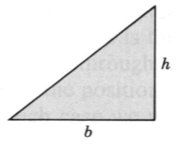
\includegraphics[width=0.35\textwidth]{graph_8.png} 
%     % \label{fig:wrapfig}
% \end{wrapfigure}
% Use integration to locate the CM of the triangular plate of base b and height h shown in the figure below.
% The plate has a uniform areal mass density $\sigma$ (mass per unit area).

% \subsection*{Solution}
% We know our equations for center of mass on the x and y axes. First, however, we calculate the formula for center of mass using area and mass density.
% \begin{align*}
%     \sigma  &=  \frac{M}{A} = \frac{dm}{dA}\\
%     dm      &=  \frac{M}{A}dA\\
%     dA      &=  \frac{A}{M}dm\\
%     x_{com} &=  \frac{1}{M}\int x\ dm
%             =   \frac{1}{A}\int x\ dA
% \end{align*}
% \begin{align*}
%     m(x) &= \sigma*x*\frac{h}{b}\\
%     x_{com} &= \frac{}{}\int_{0}^{b} \sigma*x*\frac{h}{b}\ dx 
%         = \sigma*\frac{h}{b}*\int_{0}^{b} x\ dx\\
%         &=  \sigma*\frac{h}{b}*\left[\frac{x^2}{2}\right]_0^b 
%         = \sigma*\frac{h}{b}*\frac{b^2}{2}
%         = \frac{\sigma*h*b}{2}
% \end{align*}

\end{document}